% Four original AI-generated scenes illustrate the experiment assumptions.
% Headings and captions use the deck's native typography, not bitmap text.
\begin{frame}{Perfect Communication}
  \SlideBody{%
    \centering
    {\fontsize{11}{13}\selectfont\bfseries\color{MoverDetailBlue}
      \makebox[3.6cm]{Synchronized}%
      \makebox[3.6cm]{Accurate Poses}%
      \makebox[3.6cm]{Zero Delay}%
      \makebox[3.6cm]{No Packet Loss}\par}
    \vspace{0.06cm}
    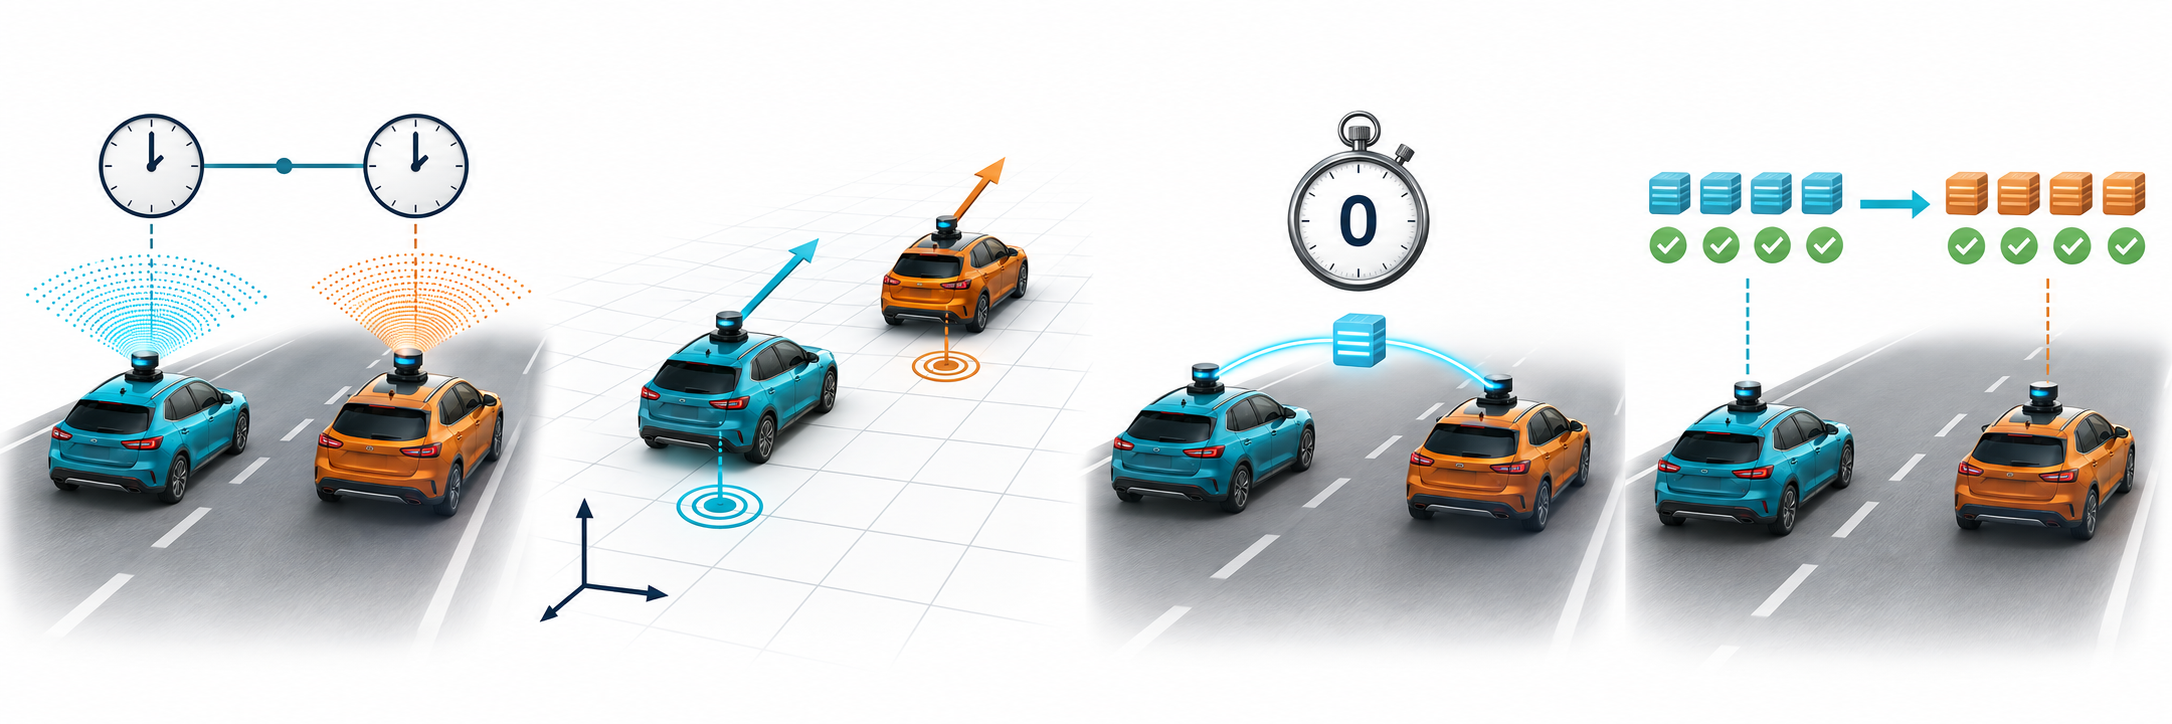
\includegraphics[width=14.4cm,height=4.80cm,keepaspectratio]{assets/illustrations/perfect-communication.png}\par
    \vspace{0.03cm}
    {\fontsize{10.5}{13}\selectfont
      % Zero-size overlays divide the four columns without moving their content.
      \makebox[0pt][l]{\hspace*{3.6cm}\raisebox{-0.05cm}[0pt][0pt]{\textcolor{MoverDetailBlue!40}{\rule{0.60pt}{5.70cm}}}}%
      \makebox[0pt][l]{\hspace*{7.2cm}\raisebox{-0.05cm}[0pt][0pt]{\textcolor{MoverDetailBlue!40}{\rule{0.60pt}{5.70cm}}}}%
      \makebox[0pt][l]{\hspace*{10.8cm}\raisebox{-0.05cm}[0pt][0pt]{\textcolor{MoverDetailBlue!40}{\rule{0.60pt}{5.70cm}}}}%
      \makebox[3.6cm]{Same observation time}%
      \makebox[3.6cm]{Position and heading}%
      \makebox[3.6cm]{0 ms latency}%
      \makebox[3.6cm]{0\% packet loss}\par}
  }
  \SlideSource{AI-generated illustration.}
\end{frame}
